\documentclass[a4paper,11pt]{report}
\usepackage[utf8]{inputenc}
\usepackage[T1]{fontenc}
\usepackage[british]{babel}
\usepackage{geometry}
\usepackage{graphicx}
\usepackage{xcolor}
\usepackage{enumitem}
\usepackage{tabularx}
\usepackage{booktabs}
\usepackage{hyperref}
\usepackage{fancyhdr}
\usepackage{lastpage}
\usepackage{tikz}
\usepackage{tcolorbox}
\usepackage{pgfplots}
\usepackage{fontawesome5}
\usepackage{multicol}

% Define DreamLab colours
\definecolor{dreamlabprimary}{RGB}{102, 51, 153}
\definecolor{dreamlabsecondary}{RGB}{255, 87, 34}
\definecolor{dreamlabaccent}{RGB}{0, 188, 212}
\definecolor{dreamlabdark}{RGB}{33, 33, 33}
\definecolor{dreamlablight}{RGB}{245, 245, 245}

% Page setup
\geometry{top=3cm, bottom=3cm, left=2.5cm, right=2.5cm}
\pagestyle{fancy}
\fancyhf{}
\fancyhead[L]{\textcolor{dreamlabprimary}{\textbf{DreamLab Go-to-Market Strategy}}}
\fancyhead[R]{\textcolor{dreamlabdark}{Page \thepage\ of \pageref{LastPage}}}
\fancyfoot[C]{\textcolor{dreamlabdark}{\small\textit{Confidential and Proprietary}}}
\renewcommand{\headrulewidth}{0.5pt}
\renewcommand{\footrulewidth}{0.3pt}

% Custom box style
\tcbset{
    dreambox/.style={
        colback=dreamlablight,
        colframe=dreamlabprimary,
        fonttitle=\bfseries,
        boxrule=2pt,
        arc=5mm,
        breakable
    },
    metricbox/.style={
        colback=dreamlabaccent!10,
        colframe=dreamlabaccent,
        fonttitle=\bfseries,
        boxrule=2pt,
        arc=3mm
    }
}

\title{
    \vspace{-2cm}
    \textcolor{dreamlabprimary}{\Huge\bfseries DreamLab}\\[0.5cm]
    \textcolor{dreamlabdark}{\Large Go-to-Market Strategy}\\[0.3cm]
    \textcolor{dreamlabsecondary}{\large Launch Plan for North-West Domination}
}
\author{\textcolor{dreamlabdark}{Strategic Marketing Team}}
\date{\textcolor{dreamlabdark}{\today}}

\begin{document}

\maketitle
\thispagestyle{empty}

\vspace{2cm}

\begin{tcolorbox}[dreambox, title=Executive Summary]
This go-to-market strategy outlines DreamLab's path to achieving £500,000 in revenue within Year 1, establishing market leadership in integrated creative technology for SMEs across the North-West. Through a phased approach combining digital marketing, strategic partnerships, and thought leadership, we will build from 2-3 pilot clients to a sustainable pipeline of recurring revenue relationships.
\end{tcolorbox}

\tableofcontents
\newpage

\chapter{Market Entry Strategy}

\section{Strategic Objectives}

\begin{tcolorbox}[dreambox, title=12-Month Goals]
\begin{enumerate}
    \item \textbf{Revenue}: Achieve £500,000 in Year 1 revenue
    \item \textbf{Client Base}: Secure 15-20 active clients across target segments
    \item \textbf{Market Position}: Establish DreamLab as top-3 creative tech agency in North-West
    \item \textbf{Recurring Revenue}: Build to 60\% recurring revenue by month 12
    \item \textbf{Brand Awareness}: Achieve 10,000 qualified contacts in CRM database
\end{enumerate}
\end{tcolorbox}

\section{Phased Launch Approach}

\subsection{Phase 1: Foundation (Months 1-3)}

\begin{table}[h]
\centering
\begin{tabularx}{\textwidth}{X|X|X}
\toprule
\textbf{Activity} & \textbf{Timeline} & \textbf{Success Metrics} \\
\midrule
Secure 2-3 pilot clients & Month 1-2 & Signed contracts \\
Build website \& core collateral & Month 1-2 & Live website, 5 case studies \\
Establish partnerships & Month 2-3 & 3 MoUs signed \\
Create content foundation & Month 2-3 & 20 pieces of content \\
Team training on GTM & Month 3 & 100\% team alignment \\
\bottomrule
\end{tabularx}
\end{table}

\subsection{Phase 2: Launch (Month 4)}

\begin{tcolorbox}[dreambox, title=Digital City Festival Launch]
\textbf{July 2025 - Major Market Entry}
\begin{itemize}
    \item Keynote presentation on ``Accessible AI for SMEs''
    \item Interactive booth demonstrating mesh fluency
    \item Launch of North-West Creative Tech Trends Report
    \item Press conference with pilot client success stories
    \item VIP reception for 50 key prospects
\end{itemize}
\end{tcolorbox}

\subsection{Phase 3: Traction (Months 5-8)}

Key activities:
\begin{itemize}
    \item Scale digital marketing campaigns
    \item Weekly thought leadership content
    \item Monthly executive roundtables
    \item Quarterly innovation workshops
    \item Strategic partnership activation
\end{itemize}

\subsection{Phase 4: Scale (Months 9-12)}

Focus areas:
\begin{itemize}
    \item National expansion planning
    \item Award submissions
    \item Client success amplification
    \item Team expansion (BD/Account Management)
    \item Series A preparation (if applicable)
\end{itemize}

\chapter{Target Market Segmentation}

\section{Primary Target Segments}

\subsection{Segment 1: Growth-Stage SMEs}

\begin{tcolorbox}[dreambox, title=Profile]
\begin{itemize}
    \item \textbf{Size}: 50-250 employees
    \item \textbf{Revenue}: £5M-£50M annually
    \item \textbf{Location}: Manchester, Liverpool, Preston, Warrington
    \item \textbf{Industries}: Manufacturing, Professional Services, Retail, Healthcare
    \item \textbf{Decision Makers}: MD/CEO, Operations Director, Digital Lead
\end{itemize}
\end{tcolorbox}

\textbf{Approach Strategy}:
\begin{itemize}
    \item LinkedIn ABM campaigns targeting leadership
    \item Industry association partnerships
    \item ROI-focused case studies
    \item Phased transformation proposals
\end{itemize}

\subsection{Segment 2: Tech Startups \& Scale-ups}

\begin{tcolorbox}[dreambox, title=Profile]
\begin{itemize}
    \item \textbf{Size}: 10-50 employees
    \item \textbf{Funding}: Seed to Series B
    \item \textbf{Location}: MediaCityUK, Baltic Triangle, Manchester Science Park
    \item \textbf{Needs}: MVP development, investor demos, rapid scaling
    \item \textbf{Decision Makers}: Founders, CTOs, Product Leads
\end{itemize}
\end{tcolorbox}

\textbf{Approach Strategy}:
\begin{itemize}
    \item Presence at startup events and accelerators
    \item Partnership with Tech Nation and local hubs
    \item Agile sprint-based engagement models
    \item Startup-friendly pricing packages
\end{itemize}

\subsection{Segment 3: Public Sector \& Cultural}

\begin{tcolorbox}[dreambox, title=Profile]
\begin{itemize}
    \item \textbf{Organisations}: Councils, NHS Trusts, Museums, Universities
    \item \textbf{Budget}: £25K-£250K per project
    \item \textbf{Process}: Formal procurement, tender-driven
    \item \textbf{Priorities}: Accessibility, social value, innovation
    \item \textbf{Decision Makers}: Procurement teams, Department heads
\end{itemize}
\end{tcolorbox}

\textbf{Approach Strategy}:
\begin{itemize}
    \item Framework agreement applications
    \item Social value documentation
    \item Pilot programme proposals
    \item Compliance-first messaging
\end{itemize}

\section{Market Sizing and Opportunity}

\begin{table}[h]
\centering
\begin{tabularx}{\textwidth}{X|r|r|r}
\toprule
\textbf{Segment} & \textbf{TAM (£)} & \textbf{SAM (£)} & \textbf{SOM Year 1 (£)} \\
\midrule
Growth SMEs & £500M & £50M & £250K \\
Tech Startups & £200M & £20M & £150K \\
Public Sector & £300M & £30M & £100K \\
\midrule
\textbf{Total} & \textbf{£1B} & \textbf{£100M} & \textbf{£500K} \\
\bottomrule
\end{tabularx}
\end{table}

\chapter{Marketing Channel Strategy}

\section{Digital Marketing Channels}

\subsection{Search Engine Marketing (SEM)}

\begin{tcolorbox}[dreambox, title=SEM Strategy]
\textbf{Organic (SEO)}:
\begin{itemize}
    \item Target keywords: ``creative agency Manchester'', ``AI consultancy North West'', ``immersive experiences UK''
    \item Content clusters around AI, immersive tech, digital transformation
    \item Local SEO optimization for ``near me'' searches
    \item Technical SEO audit and optimization monthly
\end{itemize}

\textbf{Paid (PPC)}:
\begin{itemize}
    \item Google Ads budget: £2,000/month initial
    \item Focus on high-intent commercial keywords
    \item Retargeting campaigns for website visitors
    \item LinkedIn Ads for B2B decision makers
\end{itemize}
\end{tcolorbox}

\subsection{Content Marketing}

\begin{table}[h]
\centering
\begin{tabularx}{\textwidth}{X|X|X}
\toprule
\textbf{Content Type} & \textbf{Frequency} & \textbf{Distribution} \\
\midrule
Blog Posts & 2x weekly & Website, LinkedIn, Email \\
Case Studies & 1x monthly & Website, Sales enablement \\
Video Demos & 2x monthly & YouTube, LinkedIn, Website \\
Whitepapers & Quarterly & Gated on website \\
Webinars & Monthly & Zoom, recording on YouTube \\
Podcasts & Bi-weekly & Spotify, Apple, Website \\
\bottomrule
\end{tabularx}
\end{table}

\subsection{Social Media Strategy}

\begin{itemize}
    \item \textbf{LinkedIn} (Primary):
        \begin{itemize}
            \item Daily posts from leadership team
            \item Weekly company updates
            \item Employee advocacy programme
            \item LinkedIn Live monthly demos
        \end{itemize}
    \item \textbf{Twitter/X} (Secondary):
        \begin{itemize}
            \item Industry news commentary
            \item Event live-tweeting
            \item Quick tips and insights
        \end{itemize}
    \item \textbf{Instagram} (Tertiary):
        \begin{itemize}
            \item Behind-the-scenes content
            \item Team culture posts
            \item Visual project highlights
        \end{itemize}
\end{itemize}

\subsection{Email Marketing}

\begin{tcolorbox}[dreambox, title=Email Campaigns]
\begin{enumerate}
    \item \textbf{Weekly Newsletter}: Industry insights, tips, company news (10,000 subscribers target)
    \item \textbf{Monthly Executive Brief}: C-suite focused trends and strategies
    \item \textbf{Nurture Sequences}: 
        \begin{itemize}
            \item AI Transformation (7-email series)
            \item Immersive Tech 101 (5-email series)
            \item Funding Your Innovation (6-email series)
        \end{itemize}
    \item \textbf{Event Invitations}: Workshops, webinars, roundtables
\end{enumerate}
\end{tcolorbox}

\section{Offline Marketing Channels}

\subsection{Events and Conferences}

\begin{table}[h]
\centering
\begin{tabularx}{\textwidth}{X|X|X}
\toprule
\textbf{Event Type} & \textbf{Specific Events} & \textbf{Participation Level} \\
\midrule
Major Conferences & Digital City Festival, MIPIM UK & Sponsor + Speaker \\
Industry Events & Manchester Tech Festival & Exhibitor + Workshop \\
Networking & Chamber of Commerce, Tech Manchester & Active Member \\
Own Events & DreamLab Innovation Days & Host Quarterly \\
\bottomrule
\end{tabularx}
\end{table}

\subsection{Partnership Marketing}

Key partnership targets:
\begin{itemize}
    \item \textbf{Technology Partners}: Microsoft, Google Cloud, Meta
    \item \textbf{Academic}: University of Salford, MMU, University of Manchester
    \item \textbf{Business Networks}: Manchester Digital, Downtown in Business
    \item \textbf{Accelerators}: Techstars, Ignite, Baltic Ventures
    \item \textbf{Complementary Agencies}: PR firms, traditional marketing agencies
\end{itemize}

\chapter{Campaign Strategy}

\section{Launch Campaign: ``Make the Impossible Accessible''}

\begin{tcolorbox}[dreambox, title=Campaign Overview]
\textbf{Objective}: Position DreamLab as the agency that democratises enterprise-level creative technology\\
\textbf{Duration}: 3 months (Months 4-6)\\
\textbf{Budget}: £50,000\\
\textbf{Channels}: Digital, PR, Events, Direct Marketing
\end{tcolorbox}

\subsection{Campaign Elements}

\begin{enumerate}
    \item \textbf{Hero Video}: 2-minute sizzle reel showcasing integrated capabilities
    \item \textbf{Success Stories}: 5 pilot client transformations
    \item \textbf{Interactive Demo}: ``Build Your Digital Future'' web tool
    \item \textbf{Executive Roundtables}: ``Innovation Leaders Breakfast'' series
    \item \textbf{PR Blitz}: Trade media, local business press, tech publications
\end{enumerate}

\subsection{Campaign Timeline}

\begin{figure}[h]
\centering
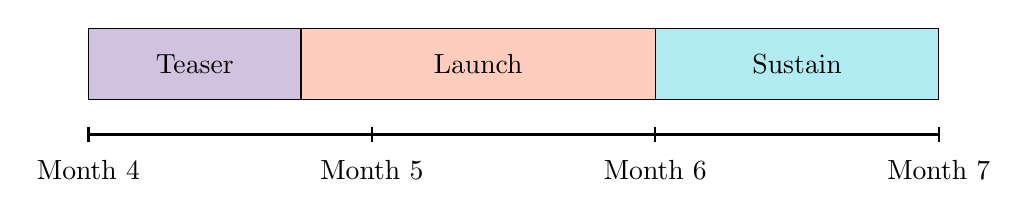
\begin{tikzpicture}[scale=0.9]
    % Timeline
    \draw[thick] (0,0) -- (12,0);
    
    % Months
    \foreach \x in {0,4,8,12} {
        \draw[thick] (\x,0.1) -- (\x,-0.1);
    }
    
    % Labels
    \node at (0,-0.5) {Month 4};
    \node at (4,-0.5) {Month 5};
    \node at (8,-0.5) {Month 6};
    \node at (12,-0.5) {Month 7};
    
    % Campaign phases
    \draw[fill=dreamlabprimary!30] (0,0.5) rectangle (3,1.5);
    \node at (1.5,1) {Teaser};
    
    \draw[fill=dreamlabsecondary!30] (3,0.5) rectangle (8,1.5);
    \node at (5.5,1) {Launch};
    
    \draw[fill=dreamlabaccent!30] (8,0.5) rectangle (12,1.5);
    \node at (10,1) {Sustain};
\end{tikzpicture}
\caption{Launch Campaign Timeline}
\end{figure}

\section{Ongoing Campaign Themes}

\subsection{Q3 2025: ``AI for Everyone''}
Focus on democratising AI for SMEs with practical use cases and ROI stories.

\subsection{Q4 2025: ``Immersive Futures''}
Showcase AR/VR applications for business transformation.

\subsection{Q1 2026: ``Creative Catalyst''}
Position DreamLab as the growth enabler for ambitious businesses.

\chapter{Sales Strategy}

\section{Sales Process}

\subsection{Lead Qualification Framework}

\begin{tcolorbox}[dreambox, title=BANT+ Criteria]
\begin{itemize}
    \item \textbf{Budget}: Minimum £10K project or £2K/month retainer capacity
    \item \textbf{Authority}: Direct access to decision maker
    \item \textbf{Need}: Clear business challenge requiring creative tech
    \item \textbf{Timeline}: Project start within 3 months
    \item \textbf{+Culture Fit}: Values innovation and partnership approach
\end{itemize}
\end{tcolorbox}

\subsection{Sales Stages}

\begin{enumerate}
    \item \textbf{Discovery Call} (30 mins)
        \begin{itemize}
            \item Understand business challenges
            \item Assess technical requirements
            \item Gauge budget and timeline
        \end{itemize}
    
    \item \textbf{Solution Workshop} (2 hours)
        \begin{itemize}
            \item Deep dive into requirements
            \item Collaborative ideation
            \item Technical feasibility assessment
        \end{itemize}
    
    \item \textbf{Proposal Presentation} (1 hour)
        \begin{itemize}
            \item Customised solution design
            \item Clear ROI projections
            \item Phased implementation plan
        \end{itemize}
    
    \item \textbf{Contract Negotiation}
        \begin{itemize}
            \item Flexible payment terms
            \item Performance guarantees
            \item Partnership agreements
        \end{itemize}
\end{enumerate}

\section{Pricing Strategy}

\subsection{Service Packaging}

\begin{table}[h]
\centering
\begin{tabularx}{\textwidth}{X|X|X|X}
\toprule
\textbf{Package} & \textbf{Price Range} & \textbf{Duration} & \textbf{Ideal For} \\
\midrule
Discovery Sprint & £5K-£15K & 2-4 weeks & New clients, problem definition \\
Transformation Project & £25K-£75K & 2-6 months & Major initiatives \\
Growth Retainer & £3K-£8K/month & Ongoing & Continuous optimisation \\
Innovation Lab & £10K-£20K & 4-6 weeks & Rapid prototyping \\
\bottomrule
\end{tabularx}
\end{table}

\subsection{Value-Based Pricing Model}

\begin{tcolorbox}[dreambox, title=Performance Incentives]
Base Fee + Performance Bonus Structure:
\begin{itemize}
    \item \textbf{E-commerce}: Base + 10\% of revenue increase
    \item \textbf{Lead Generation}: Base + £X per qualified lead
    \item \textbf{Efficiency}: Base + 15\% of cost savings
    \item \textbf{Engagement}: Base + bonus for metric improvements
\end{itemize}
\end{tcolorbox}

\chapter{Channel Partner Programme}

\section{Partner Types}

\subsection{Technology Partners}

\begin{itemize}
    \item \textbf{Platform Partners}: Shopify Plus, Adobe, Salesforce
    \item \textbf{Cloud Providers}: AWS, Google Cloud, Microsoft Azure
    \item \textbf{Software Vendors}: Unity, Unreal Engine, Meta
\end{itemize}

Benefits:
\begin{itemize}
    \item Partner directory listings
    \item Co-marketing opportunities
    \item Technical support access
    \item Certification programmes
\end{itemize}

\subsection{Referral Partners}

\begin{table}[h]
\centering
\begin{tabularx}{\textwidth}{X|X|X}
\toprule
\textbf{Partner Type} & \textbf{Referral Fee} & \textbf{Engagement Model} \\
\midrule
Business Consultants & 10\% of Year 1 revenue & Formal agreement \\
Complementary Agencies & 15\% of project value & Reciprocal referrals \\
Industry Associations & 5\% donation & Member benefits \\
Client Referrals & £1,000 per closed deal & Thank you bonus \\
\bottomrule
\end{tabularx}
\end{table}

\section{Academic Partnerships}

\begin{tcolorbox}[dreambox, title=University Collaboration Model]
\textbf{With University of Salford, MMU, University of Manchester}:
\begin{itemize}
    \item Student placement programmes (3-6 month internships)
    \item Guest lectures and workshop delivery
    \item Collaborative R\&D projects
    \item Access to innovation labs and equipment
    \item Joint funding applications (Innovate UK, UKRI)
\end{itemize}
\end{tcolorbox}

\chapter{Marketing Metrics \& KPIs}

\section{Key Performance Indicators}

\subsection{Awareness Metrics}

\begin{table}[h]
\centering
\begin{tabularx}{\textwidth}{X|r|r|r}
\toprule
\textbf{Metric} & \textbf{Month 1} & \textbf{Month 6} & \textbf{Month 12} \\
\midrule
Website Traffic & 1,000 & 5,000 & 10,000 \\
Organic Search Traffic & 100 & 1,500 & 3,500 \\
Social Media Followers & 500 & 2,500 & 5,000 \\
PR Mentions & 2 & 10 & 25 \\
Brand Search Volume & 50 & 500 & 1,500 \\
\bottomrule
\end{tabularx}
\end{table}

\subsection{Engagement Metrics}

\begin{tcolorbox}[metricbox, title=Target Engagement Rates]
\begin{itemize}
    \item Email Open Rate: 30\%+
    \item Email Click Rate: 5\%+
    \item Social Engagement Rate: 3\%+
    \item Content Download Rate: 15\%+
    \item Webinar Attendance: 40\%+
\end{itemize}
\end{tcolorbox}

\subsection{Conversion Metrics}

\begin{table}[h]
\centering
\begin{tabularx}{\textwidth}{X|X|X}
\toprule
\textbf{Funnel Stage} & \textbf{Volume Target} & \textbf{Conversion Rate} \\
\midrule
Marketing Qualified Leads (MQL) & 100/month & - \\
Sales Qualified Leads (SQL) & 25/month & 25\% \\
Opportunities Created & 10/month & 40\% \\
Deals Closed & 3/month & 30\% \\
\bottomrule
\end{tabularx}
\end{table}

\section{ROI Measurement}

\subsection{Marketing ROI Formula}

\begin{tcolorbox}[dreambox, title=ROI Calculation]
\[
\text{Marketing ROI} = \frac{\text{Revenue from Marketing} - \text{Marketing Costs}}{\text{Marketing Costs}} \times 100\%
\]

Target: 300\% ROI by Month 12
\end{tcolorbox}

\subsection{Channel Performance Tracking}

\begin{table}[h]
\centering
\begin{tabularx}{\textwidth}{X|X|X|X}
\toprule
\textbf{Channel} & \textbf{Cost/Month} & \textbf{Leads/Month} & \textbf{CPL} \\
\midrule
Organic Search & £2,000 & 30 & £67 \\
Paid Search & £2,000 & 20 & £100 \\
Social Media & £1,500 & 15 & £100 \\
Email Marketing & £500 & 25 & £20 \\
Events & £3,000 & 10 & £300 \\
\bottomrule
\end{tabularx}
\end{table}

\chapter{Marketing Technology Stack}

\section{Core Marketing Tools}

\begin{tcolorbox}[dreambox, title=MarTech Infrastructure]
\begin{itemize}
    \item \textbf{CRM}: HubSpot (CRM, Marketing, Sales, Service Hubs)
    \item \textbf{Analytics}: Google Analytics 4, Hotjar, Microsoft Clarity
    \item \textbf{SEO}: SEMrush, Screaming Frog, Google Search Console
    \item \textbf{Social Media}: Hootsuite, LinkedIn Sales Navigator
    \item \textbf{Content}: WordPress, Canva, Adobe Creative Suite
    \item \textbf{Email}: HubSpot Email, Litmus
    \item \textbf{Webinars}: Zoom Webinars, StreamYard
    \item \textbf{Project Management}: Monday.com, Slack
\end{itemize}
\end{tcolorbox}

\section{Marketing Automation Workflows}

\subsection{Lead Nurturing Automation}

\begin{enumerate}
    \item \textbf{Welcome Series}: 5-email onboarding for new subscribers
    \item \textbf{Engagement Scoring}: Automatic lead scoring based on behaviour
    \item \textbf{Re-engagement}: Win-back campaigns for inactive contacts
    \item \textbf{Event Follow-up}: Automated sequences post-webinar/event
    \item \textbf{Sales Handoff}: Automatic notification when leads are sales-ready
\end{enumerate}

\chapter{Content Strategy}

\section{Content Pillars}

\begin{tcolorbox}[dreambox, title=Core Content Themes]
\begin{enumerate}
    \item \textbf{AI Democratisation} (30\%)
        \begin{itemize}
            \item Practical AI use cases for SMEs
            \item ROI calculators and case studies
            \item Implementation guides
        \end{itemize}
    
    \item \textbf{Immersive Innovation} (25\%)
        \begin{itemize}
            \item AR/VR business applications
            \item Virtual showroom tours
            \item Metaverse readiness
        \end{itemize}
    
    \item \textbf{Creative Excellence} (25\%)
        \begin{itemize}
            \item Design thinking for business
            \item Brand transformation stories
            \item Creative campaign breakdowns
        \end{itemize}
    
    \item \textbf{Digital Transformation} (20\%)
        \begin{itemize}
            \item Step-by-step guides
            \item Technology selection advice
            \item Change management tips
        \end{itemize}
\end{enumerate}
\end{tcolorbox}

\section{Content Calendar Overview}

\subsection{Monthly Content Mix}

\begin{itemize}
    \item 8 Blog posts (2 per week)
    \item 4 Video pieces (weekly)
    \item 2 Case studies
    \item 1 Whitepaper/Guide
    \item 1 Webinar
    \item 20 Social media posts (daily)
    \item 4 Email newsletters (weekly)
\end{itemize}

\section{Thought Leadership Programme}

\subsection{Executive Visibility Plan}

\begin{table}[h]
\centering
\begin{tabularx}{\textwidth}{X|X|X}
\toprule
\textbf{Executive} & \textbf{Focus Topics} & \textbf{Channels} \\
\midrule
CEO & Vision, Industry Future & LinkedIn, Conferences \\
CTO & Technical Innovation & Tech blogs, Podcasts \\
Creative Director & Design Thinking & Instagram, YouTube \\
CMO & Marketing Innovation & Marketing publications \\
\bottomrule
\end{tabularx}
\end{table}

\chapter{Budget Allocation}

\section{Marketing Budget Breakdown}

\begin{tcolorbox}[dreambox, title=Annual Marketing Budget: £150,000]
\begin{table}[h]
\centering
\begin{tabularx}{\textwidth}{X|r|r}
\toprule
\textbf{Category} & \textbf{Amount (£)} & \textbf{\% of Budget} \\
\midrule
Digital Marketing & 60,000 & 40\% \\
Events \& Conferences & 30,000 & 20\% \\
Content Creation & 25,000 & 17\% \\
PR \& Communications & 15,000 & 10\% \\
Marketing Technology & 10,000 & 7\% \\
Partnerships & 5,000 & 3\% \\
Contingency & 5,000 & 3\% \\
\midrule
\textbf{Total} & \textbf{150,000} & \textbf{100\%} \\
\bottomrule
\end{tabularx}
\end{table}
\end{tcolorbox}

\section{ROI Projections}

\begin{table}[h]
\centering
\begin{tabularx}{\textwidth}{X|r|r|r}
\toprule
\textbf{Quarter} & \textbf{Marketing Spend} & \textbf{Revenue Generated} & \textbf{ROI} \\
\midrule
Q1 (Launch) & £50,000 & £75,000 & 50\% \\
Q2 & £35,000 & £125,000 & 257\% \\
Q3 & £35,000 & £150,000 & 329\% \\
Q4 & £30,000 & £150,000 & 400\% \\
\midrule
\textbf{Year 1 Total} & \textbf{£150,000} & \textbf{£500,000} & \textbf{233\%} \\
\bottomrule
\end{tabularx}
\end{table}

\chapter{Risk Management}

\section{Marketing Risks and Mitigation}

\begin{table}[h]
\centering
\begin{tabularx}{\textwidth}{X|X|X}
\toprule
\textbf{Risk} & \textbf{Impact} & \textbf{Mitigation} \\
\midrule
Low brand awareness & Slow lead generation & Aggressive PR, partnerships \\
Competition response & Price pressure & Focus on unique value prop \\
Economic downturn & Reduced budgets & Flexible pricing, ROI focus \\
Talent shortage & Delivery issues & Partner network, freelancers \\
Technology changes & Service obsolescence & Continuous learning, R\&D \\
\bottomrule
\end{tabularx}
\end{table}

\section{Contingency Planning}

\begin{tcolorbox}[dreambox, title=Scenario Planning]
\textbf{Best Case} (120\% of target):
\begin{itemize}
    \item Accelerate hiring
    \item Increase marketing spend
    \item Expand geographically faster
\end{itemize}

\textbf{Base Case} (100\% of target):
\begin{itemize}
    \item Execute plan as outlined
    \item Maintain steady growth
    \item Build for Year 2 expansion
\end{itemize}

\textbf{Worst Case} (70\% of target):
\begin{itemize}
    \item Reduce paid marketing
    \item Focus on referrals
    \item Extend runway through cost control
\end{itemize}
\end{tcolorbox}

\chapter{Implementation Timeline}

\section{90-Day Quick Wins}

\begin{tcolorbox}[dreambox, title=Immediate Actions]
\textbf{Days 1-30}:
\begin{itemize}
    \item Launch website with core messaging
    \item Set up marketing automation
    \item Begin content production
    \item Secure Digital City Festival slot
\end{itemize}

\textbf{Days 31-60}:
\begin{itemize}
    \item Launch paid search campaigns
    \item Publish first case studies
    \item Host inaugural webinar
    \item Activate partnership discussions
\end{itemize}

\textbf{Days 61-90}:
\begin{itemize}
    \item PR launch announcement
    \item First executive roundtable
    \item Email nurture campaigns live
    \item Sales enablement tools ready
\end{itemize}
\end{tcolorbox}

\section{Year 1 Marketing Calendar}

\begin{table}[h]
\centering
\small
\begin{tabularx}{\textwidth}{l|X}
\toprule
\textbf{Month} & \textbf{Key Activities} \\
\midrule
Month 1 & Foundation building, pilot client acquisition \\
Month 2 & Content creation, website development \\
Month 3 & Partnership establishment, team training \\
Month 4 & Digital City Festival launch, PR blitz \\
Month 5 & Campaign optimisation, lead nurturing \\
Month 6 & Thought leadership push, awards entries \\
Month 7 & Summer events, client success stories \\
Month 8 & Autumn campaign planning, team expansion \\
Month 9 & Conference season, partnership activation \\
Month 10 & Q4 push, year-end planning \\
Month 11 & Black Friday tech offers, case studies \\
Month 12 & Year review, 2026 planning \\
\bottomrule
\end{tabularx}
\end{table}

\appendix

\chapter{Marketing Templates}

\section{Campaign Brief Template}

\begin{tcolorbox}[dreambox, title=Campaign Planning Framework]
\textbf{Campaign Name}: [Insert name]\\
\textbf{Objective}: [SMART goal]\\
\textbf{Target Audience}: [Specific segment]\\
\textbf{Key Message}: [One clear statement]\\
\textbf{Channels}: [List all channels]\\
\textbf{Budget}: [Total and breakdown]\\
\textbf{Timeline}: [Start and end dates]\\
\textbf{Success Metrics}: [3-5 KPIs]\\
\textbf{Creative Assets Needed}: [List all materials]\\
\textbf{Team Responsibilities}: [RACI matrix]
\end{tcolorbox}

\section{Lead Scoring Model}

\begin{table}[h]
\centering
\begin{tabularx}{\textwidth}{X|c|X}
\toprule
\textbf{Behaviour} & \textbf{Points} & \textbf{Rationale} \\
\midrule
Downloaded whitepaper & +10 & Shows research intent \\
Attended webinar & +15 & High engagement \\
Visited pricing page & +20 & Commercial intent \\
Opened 5+ emails & +5 & Consistent interest \\
C-suite title & +25 & Decision maker \\
Company size 50+ & +15 & Ideal customer profile \\
Requested demo & +30 & High intent \\
\midrule
\multicolumn{3}{l}{\textbf{Threshold}: 50+ points = Sales Qualified Lead} \\
\bottomrule
\end{tabularx}
\end{table}

\chapter{Competitive Response Playbook}

\section{Competitor Monitoring}

\begin{itemize}
    \item Weekly competitor content review
    \item Monthly pricing analysis
    \item Quarterly capability comparison
    \item Win/loss analysis documentation
    \item Client feedback on alternatives
\end{itemize}

\section{Differentiation Messaging}

\begin{tcolorbox}[dreambox, title=Key Differentiators to Emphasise]
When competitors position on single capabilities, we emphasise:
\begin{itemize}
    \item \textbf{Integration}: ``Unlike agencies that only do X, we seamlessly combine AI, immersive, and creative''
    \item \textbf{Accessibility}: ``Enterprise capabilities at SME-friendly prices''
    \item \textbf{Partnership}: ``We're not just vendors, we're growth partners''
    \item \textbf{Local}: ``North-West based, globally capable''
    \item \textbf{Results}: ``Performance-based pricing aligns our success with yours''
\end{itemize}
\end{tcolorbox}

\end{document}